\section{\texorpdfstring{Třístavový výstup a sběrnice}{Tristavovy vystup a sbernice}}

% =====================================================================================================================
	\begin{frame}
    \frametitle{Sběrnice}
	
		Soustava vodičů propojující mezi sebou dva nebo více elektronických systémů:
		
		\begin{itemize}
			\item Napájecí sběrnice,
			\item adresová sběrnice,
			\item datová atd.
		\end{itemize}
		
		\vspace{3mm}
		Rozlišujeme dva druhy zařízení na sběrnici:
		
		\begin{description}
			\item[\textbf{vysílač}] - nastavuje a udržuje signál na sběrnici,
			\item[\textbf{přijímač}] - čte signál na sběrnici a reaguje na něj.
		\end{description}
		
		\vspace{3mm}
		Sběrnice může mít několik vysílačů. Řešíme tak problém kolize výstupů, protože nelze připojit dva a více výstupů dohromady na jeden vodič.
		
	\end{frame}
	
% =====================================================================================================================
	\begin{frame}
    \frametitle{Sběrnice - kolize výstupů}
	
		\begin{center}
			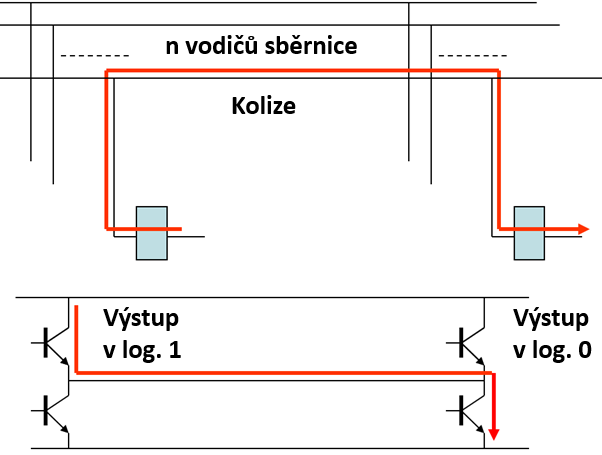
\includegraphics[scale=0.5]{fig/bus.png}
		\end{center}
		
	\end{frame}
	
% =====================================================================================================================
	\begin{frame}
    \frametitle{Třístavový buffer}
		\small
		
		
		\begin{minipage}[t][\textheight][t]{0.4\textwidth}
		\vspace{5mm}
		\textbf{Symbol:}
		\begin{center}
			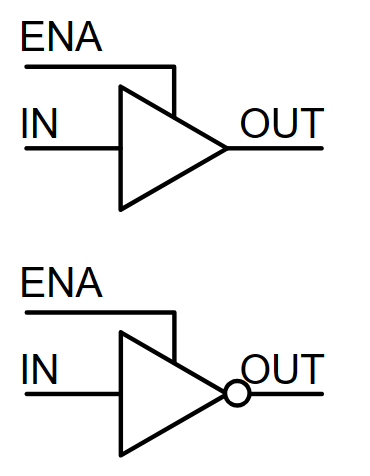
\includegraphics[width=0.50\textwidth]{fig/3state_buffer.png}
		\end{center}
			
		\end{minipage}
		\begin{minipage}[t][\textheight][t]{0.55\textwidth}
		
		\begin{itemize}
			\item Kromě dvou výstupních stavů logické 0 a logické 1 nabízí stav vysoké impedance,
			\item stavy se obvykle značí 0, 1, Z nebo L, H, Z,
			\item lze se setkat i s verzí s invertorem,
			\item na místě třístavového výstupu lze někdy použít hradla s otevřeným kolektorem.
		\end{itemize}
		
		\vspace{1mm}
		\begin{center}
			\begin{tabular}{c c | c}
				$ENA$ & $IN$ & $OUT$ \\ 
				\hline
				$0$ & $0$ & $Z$ \\
				$0$ & $1$ & $Z$ \\
				$1$ & $0$ & $0$ \\
				$1$ & $1$ & $1$ \\
			\end{tabular}
		\end{center}
		
		\end{minipage}
	\end{frame}
	
% =====================================================================================================================
	\begin{frame}
    \frametitle{Multiplexer pro sběrnici}
		
		\begin{center}
			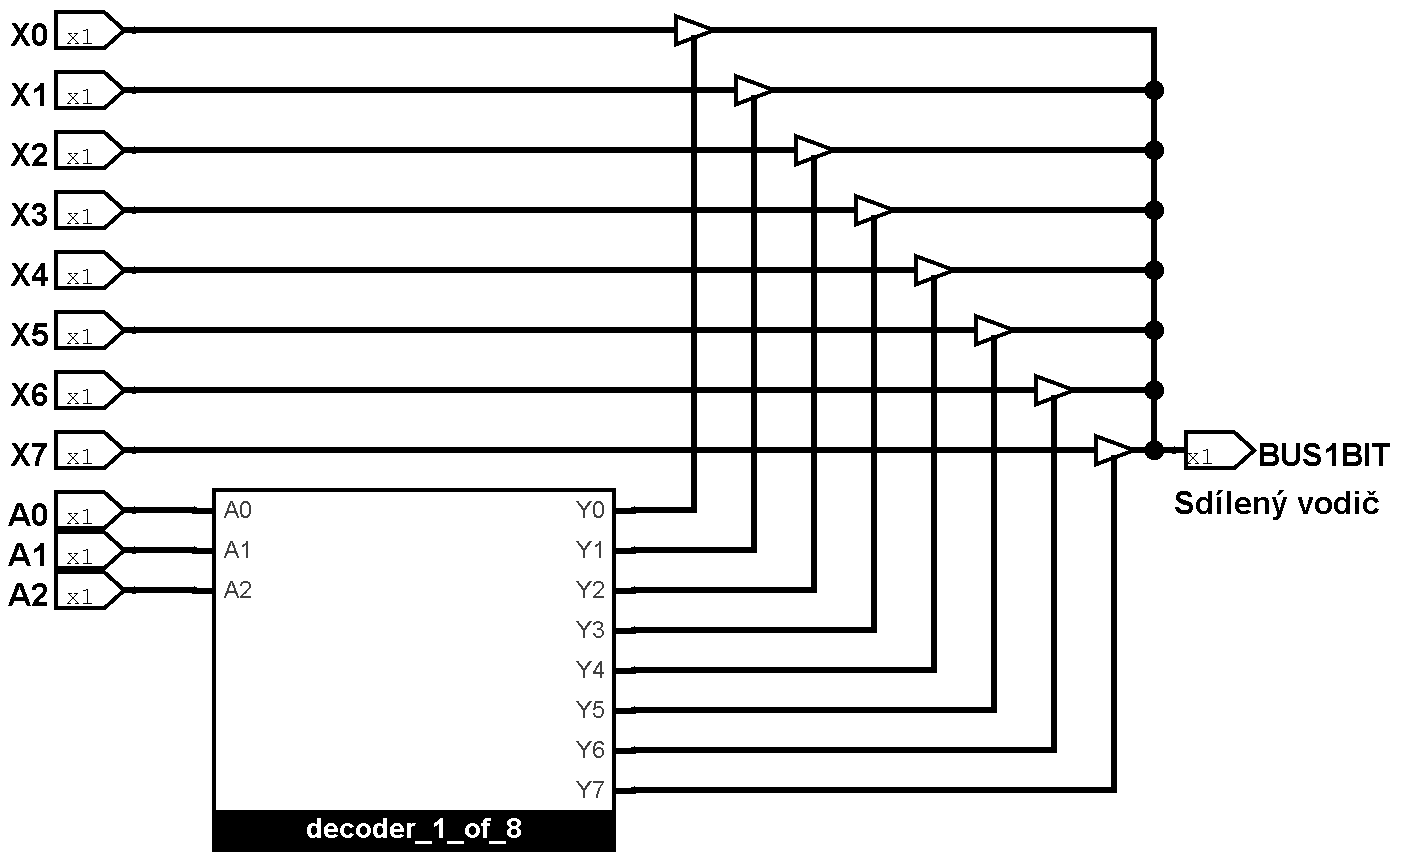
\includegraphics[width=0.90\textwidth]{fig/mux_8_bus.png}
		\end{center}
		
	\end{frame}
	
% =====================================================================================================================
	\begin{frame}
    \frametitle{Sběrnice - otevřený kolektor}
	
		\begin{center}
			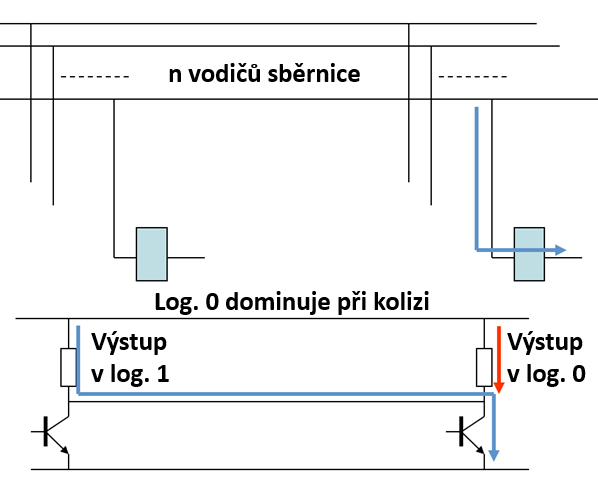
\includegraphics[scale=0.5]{fig/bus_open_colector.png}
		\end{center}
		
	\end{frame}
		
% =====================================================================================================================
	\begin{frame}
    \frametitle{Příklad výstupu mikroprocesoru STM8S208}
	
		\begin{center}
			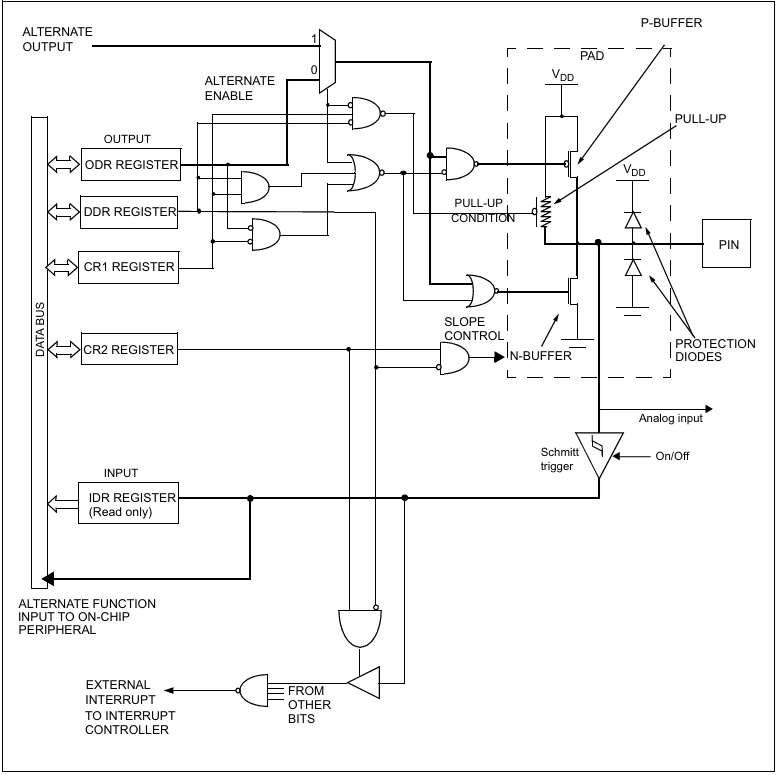
\includegraphics[height=0.85\textheight]{fig/gpio_stm8.png}
		\end{center}
		
	\end{frame}